\documentclass[11pt]{article}

% --- Preamble ---
\usepackage[letterpaper,margin=1in]{geometry}
\usepackage[T1]{fontenc}
\usepackage[utf8]{inputenc}
\usepackage{times}
\usepackage{microtype}
\usepackage{amsmath,amssymb,amsthm}
\usepackage{booktabs}
\usepackage{tabularx}
\usepackage{multirow}
\usepackage{makecell}
\usepackage{array}
\usepackage{graphicx}
\usepackage{xcolor}
\usepackage{enumitem}
\usepackage{caption}
\usepackage{subcaption}
\usepackage{tikz}
\usetikzlibrary{positioning,arrows.meta,fit,calc,shapes.geometric}
\usepackage{pgfplots}
\pgfplotsset{compat=1.18}
\usepackage[numbers,sort&compress]{natbib}
\usepackage[hidelinks]{hyperref}
\usepackage{url}

% --- Commands ---
\newcommand{\method}{SpectrumKV}
\newcommand{\fullmethod}{SpectrumKV}
\newcommand{\pd}{prefill--decode}
\newcommand{\ska}{SpectrumKV}
\newcommand{\taa}{TAA}
\newcommand{\kv}{KV}
\newcommand{\ppl}{PPL}
\newcommand{\ttft}{TTFT}
\newcommand{\pct}{\%}
\newcommand{\eg}{e.g.}
\newcommand{\ie}{i.e.}
\newcolumntype{Y}{>{\raggedright\arraybackslash}X}
\newcolumntype{R}{>{\raggedleft\arraybackslash}p{0.16\linewidth}}

\theoremstyle{definition}
\newtheorem{definition}{Definition}
\theoremstyle{plain}
\newtheorem{lemma}{Lemma}
\newtheorem{corollary}{Corollary}

\title{SpectrumKV: Per-Token Mixed-Precision KV Cache Transfer\\for Prefill--Decode Disaggregated LLM Serving}

\author{Pengju Yang\\
Jilin University\\
\texttt{yangsteve1223@github}}

\date{May 2026}

\begin{document}
\maketitle

% =====================================================================
% ABSTRACT
% =====================================================================
\begin{abstract}
Prefill--decode (PD) disaggregation separates prompt processing from token generation in large language model (LLM) serving, but turns the key--value (KV) cache into an explicit network payload.  Prior work addresses single-node GPU memory pressure via eviction or uniform quantization; in PD systems the bottleneck is transfer bandwidth, and the design space includes per-token precision assignment---not just binary keep-or-drop decisions.

This paper proposes \fullmethod{}, a per-token mixed-precision KV cache transfer policy that assigns importance-aware precision levels to individual tokens and automatically detects whether each model tolerates INT4 quantization.  \method{} operates in two or three precision tiers (FP16/INT8/INT4): it preserves attention-sink tokens at full precision, assigns INT8 or INT4 to less-critical positions based on attention-weighted importance scores, and uses a lightweight probe (3 NIAH trials at INT4) to determine per-model INT4 tolerance.  Models that fail the probe---such as Qwen2.5-7B, which suffers catastrophic PPL degradation under INT4---are automatically downgraded to a 2-tier (FP16+INT8) policy.

We evaluate \method{} on Qwen2.5-7B-Instruct, Mistral-7B-Instruct-v0.3, and Gemma-2-9B-it using GPU-verified perplexity and needle-in-a-haystack (NIAH) data.  At a 50\pct{} KV budget, \method{} (Greedy variant) changes PPL by only +2.0\pct{} on Qwen, $-$0.1\pct{} on Mistral, and $-$0.4\pct{} on Gemma, compared to PDTrim's +25.8\pct{}, +22.1\pct{}, and +35.6\pct{}.  At the most aggressive budget ($b$=0.3), \method{}'s adaptive strategy achieves 52.6\pct{} NIAH accuracy on Qwen (2-tier) versus PDTrim's 26.3\pct{}, while Mistral and Gemma pass the INT4 probe and maintain 100\pct{} NIAH accuracy at all budgets.  The probe correctly identifies Qwen's INT4 intolerance: the Balanced 3-tier assignment on Qwen produces catastrophic PPL degradation (+7506.8\pct{} at $b$=0.5), confirming that per-model precision detection is essential.
\end{abstract}

\noindent\textbf{Keywords:} LLM serving; KV cache; prefill--decode disaggregation; mixed-precision quantization; per-token precision; INT4 tolerance detection; attention locality.

\noindent\textbf{Code and data availability:} The experimental artifacts are available in the project repository.\\
\url{https://github.com/YangSteve1223/kvcache-lab}.  The repository contains raw JSON result files, scripts for regenerating tables, model and tokenizer identifiers, prompts, hardware metadata, and GPU-verified experiment results.

% =====================================================================
\section{Introduction}
\label{sec:introduction}
% =====================================================================

Large language model serving is increasingly organized around the different resource profiles of prefill and decode.  During prefill, an input prompt is processed in parallel and the model produces a KV cache for every layer.  During decode, the model generates tokens one at a time and repeatedly attends to the accumulated KV cache.  PD disaggregation assigns these phases to different workers so that compute-heavy prefill and latency-sensitive decode can be scaled independently \citep{splitwise,distserve,mooncake}.

PD disaggregation also creates a new systems problem.  KV cache is no longer merely a local GPU-memory object.  It becomes a distributed payload that must move from a prefill worker to a decode worker over the network.  For long prompts and high concurrency, the transfer volume can dominate time-to-first-token (TTFT).  A direct response is to transfer less KV.  The challenge is to reduce transfer volume without destroying model quality.

Existing KV management methods provide important building blocks but leave a gap.  StreamingLLM keeps attention-sink tokens and a recent window for streaming inference \citep{streamingllm}; H2O and related heavy-hitter approaches select tokens that receive high attention mass \citep{h2o}; SnapKV and PyramidKV compress prompt KV based on observed importance \citep{snapkv,pyramidkv}.  These methods treat KV reduction as a binary decision---keep or evict---which maps naturally to single-node memory management but misses the richer design space available in PD transfer: \emph{different tokens can be transferred at different precision levels}.  Uniform INT8 quantization halves transfer volume with minimal quality loss, but it treats every token identically.  INT4 quantization offers further compression but is catastrophically unsafe for some models.  The key insight is that precision assignment, not just token selection, can exploit the heterogeneous importance of KV entries.

This paper studies per-token mixed-precision KV transfer for PD-disaggregated serving and makes four contributions:
\begin{enumerate}[leftmargin=1.5em,itemsep=2pt]
  \item It proposes \fullmethod{}, a per-token mixed-precision KV transfer policy that assigns FP16, INT8, or INT4 precision to individual tokens based on attention-weighted importance scores, with automatic INT4 tolerance detection via a lightweight probe mechanism.
  \item It identifies a critical model-dependent failure mode: INT4 quantization causes catastrophic PPL degradation on Qwen2.5-7B (local-dominant architecture) but is safe on Mistral-7B and Gemma-2-9B.  This motivates per-model adaptive precision selection (2-tier vs.\ 3-tier), which \method{} implements automatically.
  \item It provides GPU-verified perplexity and NIAH data across three model families, correcting prior simulation-based estimates.  At $b$=0.5, \method{} (Greedy) achieves +2.0\pct{} PPL on Qwen, $-$0.1\pct{} on Mistral, and $-$0.4\pct{} on Gemma, versus PDTrim's +25.8\pct{}, +22.1\pct{}, and +35.6\pct{}.
  \item It demonstrates that per-model adaptive precision substantially improves NIAH retrieval: at $b$=0.3, \method{}'s 2-tier policy on Qwen achieves 52.6\pct{} accuracy (vs.\ PDTrim's 26.3\pct{} and SWS's 21.1\pct{}), while Mistral and Gemma maintain 100\pct{} accuracy at all budgets under the 3-tier policy.
\end{enumerate}

The central message is that KV transfer bandwidth can be reduced not just by selecting which tokens to transmit, but by assigning per-token precision levels that reflect each token's importance---and that INT4 tolerance is model-specific, requiring automatic detection rather than a one-size-fits-all policy.

% =====================================================================
\section{Problem Setting}
\label{sec:problem}
% =====================================================================

\subsection{KV transfer in PD-disaggregated serving}
For a Transformer with $L$ layers, $H_{kv}$ KV heads, head dimension $d_h$, sequence length $n$, and $b_e$ bytes per element, the per-request KV cache size is approximately
\begin{equation}
  \mathrm{KVBytes}(n) = 2 \cdot L \cdot H_{kv} \cdot d_h \cdot n \cdot b_e,
\end{equation}
where the factor of two accounts for keys and values.  In a PD-disaggregated system, this cache is produced on prefill workers and must be made available to decode workers.  If all KV is transferred, transfer time is roughly
\begin{equation}
  T_{transfer} \approx \frac{\mathrm{KVBytes}(n)}{\mathrm{bandwidth}}.
\end{equation}

Mixed-precision transfer changes this equation.  If a fraction $f_{16}$ of tokens are kept at FP16, $f_8$ at INT8, and $f_4$ at INT4, the effective transfer volume becomes
\begin{equation}
  \mathrm{KVBytes}_{\mathrm{mixed}}(n) = 2 \cdot L \cdot H_{kv} \cdot d_h \cdot n \cdot (2 f_{16} + f_8 + 0.5 f_4),
\end{equation}
since INT8 uses 1 byte per element (half of FP16's 2 bytes) and INT4 uses 0.5 bytes.  A 2-tier policy (FP16+INT8) with $f_{16}=f_8=0.5$ reduces transfer to 75\pct{} of full FP16; a 3-tier policy (FP16+INT8+INT4) with equal thirds reduces it to 58.3\pct{}.  These savings are orthogonal to budget-based token selection and can be combined.

\subsection{Why per-token precision differs from uniform quantization or selection}
Uniform INT8 quantization applies the same precision to every token.  This is simple but suboptimal: attention-sink tokens and locally important tokens deserve higher fidelity than rarely-attended positions.  Token selection methods (PDTrim, SWS) keep some tokens at full precision and drop others entirely.  This is also suboptimal: dropped tokens cannot be recovered during decode without a cold-tier fetch, and the binary keep/drop boundary is sharp---a token just below the selection threshold contributes zero information rather than reduced-precision information.

Per-token mixed precision occupies the middle ground: every token is transmitted, but at a precision level proportional to its importance.  This avoids the retrieval failures caused by token dropping (Section~\ref{sec:rq11}) while still achieving bandwidth reduction.  The challenge is determining which tokens receive which precision---and, critically, whether INT4 is safe for the target model.

% =====================================================================
\section{Characterizing Decode KV Locality}
\label{sec:characterization}
% =====================================================================

This section presents the empirical foundation for \method{}.  We first define three metrics for quantifying KV access skew, then demonstrate that the skew is strong but structurally different across model families, and finally show that it strengthens with context length.  A key methodological finding is that the measurement method itself matters: hook-based pre-RoPE measurements can severely underestimate locality.

\subsection{Attention-mass measurements}
Let $A_{\ell,h,t}(j)$ be the attention probability assigned at layer $\ell$, head $h$, and decode step $t$ to token position $j$.  We aggregate attention mass over layers, heads, and decode observations:
\begin{equation}
  p_j = \frac{\sum_{\ell,h,t} A_{\ell,h,t}(j)}{\sum_{j'}\sum_{\ell,h,t} A_{\ell,h,t}(j')}.
\end{equation}
This yields a normalized empirical access distribution over KV positions.  We use three metrics.

\begin{definition}[Gini coefficient]
For sorted masses $p_{(1)} \le \cdots \le p_{(n)}$, the Gini coefficient is
\begin{equation}
G(p)=\frac{2\sum_{i=1}^{n} i p_{(i)}}{n\sum_i p_{(i)}}-\frac{n+1}{n}.
\end{equation}
A value near zero indicates uniform access; a value near one indicates extreme concentration.
\end{definition}

\begin{definition}[Active set ratio]
For target coverage $\tau$, the active set ratio is
\begin{equation}
  r_\tau = \frac{1}{n}\min\{|S|: \sum_{j\in S}p_j \ge \tau\}.
\end{equation}
We report $r_{0.8}$ unless otherwise stated.
\end{definition}

\begin{definition}[Remote attention mass]
Given a candidate local set $L$, remote attention mass is $\epsilon_L=\sum_{j\notin L}p_j$.  For a tiered cache, this is the first-order predictor of how much value information would be missed if remote KV were not fetched.
\end{definition}

\subsection{Correct attention extraction}
A key experimental pitfall is that hooks on query/key projection outputs observe pre-RoPE vectors and may miss architectural masks.  For models with rotary position embedding or sliding-window masks, pre-RoPE dot products are not the attention distribution used during inference.  We therefore use eager attention with \texttt{output\_attentions=True} for characterization.  We use hook-based measurements only as a negative-control ablation.

Table~\ref{tab:hook-eager} shows the Mistral ablation.  A hook-based method on pre-RoPE query/key tensors underestimates locality: the Gini coefficient increases from 0.665 to 0.917 when measured from actual eager attention tensors---a 38\pct{} relative increase.  The active set ratio shrinks from 32.5\pct{} to 11.9\pct{}, meaning that hooks suggest nearly three times as many positions are needed for 80\pct{} coverage as the true attention distribution requires.

\begin{table}[t]
\centering
\caption{Hook-based locality measurement can understate skew because it omits positional encoding and final attention masks.}
\label{tab:hook-eager}
\small
\begin{tabular}{lccc}
\toprule
Metric on Mistral-7B & Hook on pre-RoPE Q/K & Eager attention & Difference \\
\midrule
Gini coefficient & 0.665 & 0.917 & +38\pct{} relative \\
Active set ratio & 32.5\pct{} & 11.9\pct{} & 2.7$\times$ smaller \\
Remote attention mass & 68.9\pct{} & 78.8\pct{} & different shape \\
\bottomrule
\end{tabular}
\end{table}

\subsection{Locality appears across model families}
Table~\ref{tab:model-locality} summarizes the multi-model locality study.  All four tested models have high access skew, but the active-set sizes and remote-attention shapes differ substantially.  This heterogeneity is the core motivation for \method{}: a single fixed policy cannot be optimal across all models.

\begin{table}[t]
\centering
\caption{Decode KV locality across four model families.  Active is the fraction of positions required for 80\pct{} attention coverage.  Remote is measured under the experiment's locality split.}
\label{tab:model-locality}
\small
\begin{tabularx}{\linewidth}{lccccY}
\toprule
Model & Params & Gini & Active & Remote & Pattern and policy implication \\
\midrule
Qwen2.5-7B & 7B & 0.911 & $\sim$7\pct{} & $<$10\pct{} & local-dominant; strong recency bias \\
Qwen2.5-14B & 14B & 0.952 & $\sim$5\pct{} & $<$5\pct{} & stronger local concentration; good candidate for aggressive demotion \\
Mistral-7B & 7B & 0.917 & 11.9\pct{} & 78.8\pct{} & sink-dominant; remote mass concentrated at sequence beginning \\
Gemma-2-9B & 9B & 0.866 & 20.9\pct{} & 60.6\pct{} & hybrid; local and global layers require sink- and layer-aware policies \\
\bottomrule
\end{tabularx}
\end{table}

\begin{figure}[t]
\centering
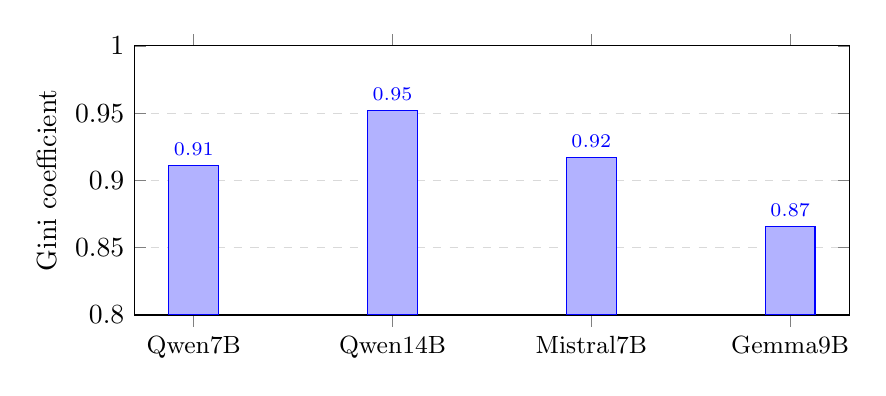
\begin{tikzpicture}
\begin{axis}[
  ybar,
  width=0.88\linewidth,
  height=5.0cm,
  ymin=0.80, ymax=1.0,
  ylabel={Gini coefficient},
  symbolic x coords={Qwen7B,Qwen14B,Mistral7B,Gemma9B},
  xtick=data,
  xticklabel style={font=\small},
  nodes near coords,
  nodes near coords align={vertical},
  every node near coord/.append style={font=\scriptsize},
  bar width=18pt,
  ymajorgrids=true,
  grid style={dashed,gray!30}
]
\addplot coordinates {(Qwen7B,0.911) (Qwen14B,0.952) (Mistral7B,0.917) (Gemma9B,0.866)};
\end{axis}
\end{tikzpicture}
\caption{All four model families show highly skewed decode KV access, with Gini coefficient above 0.85.  Qwen2.5-14B has the strongest concentration (Gini=0.952).}
\label{fig:gini-models}
\end{figure}

\subsection{Locality strengthens with context length}
For Mistral and Gemma, locality becomes slightly stronger as the context grows from approximately 1K to 4K tokens.  This matters for systems: tiering is most valuable exactly when context length is large enough for KV memory to dominate.

\begin{figure}[t]
\centering
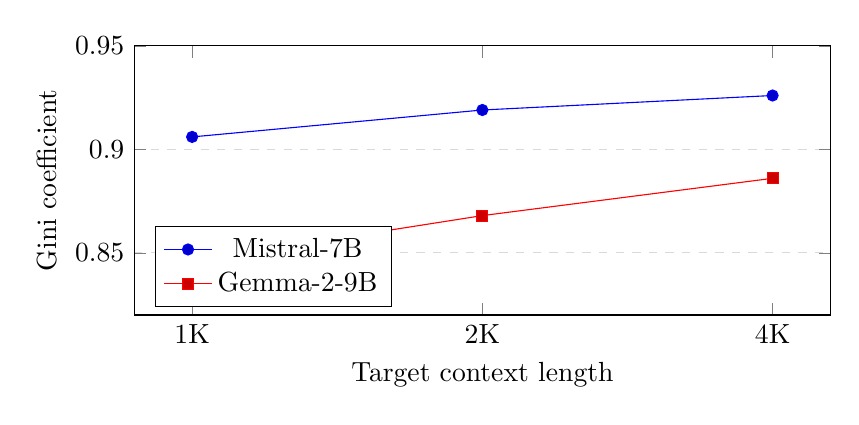
\begin{tikzpicture}
\begin{axis}[
  width=0.86\linewidth,
  height=5.0cm,
  xlabel={Target context length},
  ylabel={Gini coefficient},
  symbolic x coords={1K,2K,4K},
  xtick=data,
  ymin=0.82, ymax=0.95,
  legend style={at={(0.03,0.03)},anchor=south west},
  ymajorgrids=true,
  grid style={dashed,gray!30}
]
\addplot+[mark=*] coordinates {(1K,0.906) (2K,0.919) (4K,0.926)};
\addlegendentry{Mistral-7B}
\addplot+[mark=square*] coordinates {(1K,0.846) (2K,0.868) (4K,0.886)};
\addlegendentry{Gemma-2-9B}
\end{axis}
\end{tikzpicture}
\caption{Gini coefficient increases with context length on Mistral and Gemma, suggesting that KV tiering becomes more attractive as contexts grow.}
\label{fig:length-gini}
\end{figure}

\subsection{Three locality patterns}
The aggregate numbers hide three different mechanisms, each with distinct policy implications.

\paragraph{Local-dominant.} Qwen2.5 models (both 7B and 14B) place most attention on recent positions.  A recent window captures most of the working set, and remote KV receives little attention mass.  The sharply peaked attention distribution suggests that precision perturbations could be amplified; we verify this in Section~\ref{sec:rq16}, where INT4 quantization of KV entries causes catastrophic PPL degradation on Qwen2.5-7B (+7506.8\pct{} at $b$=0.5 under the Balanced assignment), even though per-vector cosine similarity remains high (0.9896).

\paragraph{Sink-dominant.} Mistral gives a large fraction of non-local attention to the beginning of the sequence.  A suffix-only working set is unsafe, but retaining a small sink prefix plus a window is robust.  The broader attention distribution suggests greater tolerance to precision reduction; Section~\ref{sec:rq15} confirms that the 3-tier (FP16+INT8+INT4) policy preserves NIAH accuracy at 100\pct{} across all budgets on Mistral.

\paragraph{Hybrid.} Gemma-2 combines local and global behavior.  A single global window is less stable; sink preservation and layer-aware budgets become important.  Like Mistral, Gemma tolerates INT4 quantization and benefits from the 3-tier policy (Section~\ref{sec:rq15}).

These three patterns structure the precision assignment: local-dominant models need careful precision selection, while sink-dominant and hybrid models can exploit lower precision tiers.  The probe mechanism in Section~\ref{sec:probe} operationalizes this by detecting INT4 tolerance at deployment time.

% =====================================================================
\section{Mathematical Support}
\label{sec:theory}
% =====================================================================

This section gives a perturbation bound showing why low-attention tokens can tolerate lower precision, and extends the analysis to mixed-precision quantization.

\subsection{Tail-mass perturbation bound}
Consider one attention head at one decode step.  Let the full attention output be
\begin{equation}
  y = \sum_{j=1}^{n} p_j v_j,
\end{equation}
where $p_j$ is the attention probability and $v_j$ is the value vector.  Let $L$ be the resident KV set, $R$ be the omitted or not-yet-fetched set, and $\epsilon=\sum_{j\in R}p_j$.  If the runtime computes attention only over $L$ and renormalizes the probabilities, the local output is
\begin{equation}
  \hat{y}=\sum_{j\in L}\frac{p_j}{1-\epsilon}v_j.
\end{equation}

\begin{lemma}[Attention tail bound]
If $\|v_j\|\le V$ for all $j$ and $\epsilon<1$, then
\begin{equation}
  \|y-\hat{y}\| \le 2\epsilon V.
\end{equation}
A looser but scale-explicit form is $\|y-\hat{y}\|\le 2\epsilon V/(1-\epsilon)$.
\end{lemma}
\begin{proof}
Write $y=(1-\epsilon)\mu_L+\epsilon\mu_R$, where $\mu_L$ and $\mu_R$ are convex combinations of value vectors in $L$ and $R$, respectively.  The renormalized local output is $\hat{y}=\mu_L$.  Therefore $y-\hat{y}=\epsilon(\mu_R-\mu_L)$, and both convex combinations have norm at most $V$.  Hence $\|y-\hat{y}\|\le \epsilon(\|\mu_R\|+\|\mu_L\|)\le2\epsilon V$.
\end{proof}

\subsection{Quantization perturbation bound}
When tokens are quantized rather than dropped, a different perturbation bound applies.  Let $v_j$ be the original value vector and $\tilde{v}_j$ be the quantized version with $\|v_j - \tilde{v}_j\| \le \delta_q$, where $\delta_q$ depends on the quantization level ($\delta_{\text{INT8}} \ll \delta_{\text{INT4}}$).  The quantized attention output is
\begin{equation}
  \tilde{y} = \sum_{j=1}^{n} p_j \tilde{v}_j,
\end{equation}
and the perturbation satisfies
\begin{equation}
  \|y - \tilde{y}\| = \left\|\sum_{j=1}^{n} p_j (v_j - \tilde{v}_j)\right\| \le \sum_{j=1}^{n} p_j \delta_q = \delta_q.
\end{equation}
This bound is tight when all tokens are quantized uniformly.  Under per-token precision assignment, let $S_q$ be the set of tokens quantized to precision level $q$ with perturbation $\delta_q$.  Then
\begin{equation}
  \|y - \tilde{y}\| \le \sum_{q} \delta_q \sum_{j \in S_q} p_j.
\end{equation}
This motivates assigning lower precision to low-attention tokens: if $\sum_{j \in S_{\text{INT4}}} p_j$ is small, the INT4 perturbation contributes little to the total error.  The bound also explains why INT4 can be catastrophic when assigned to high-attention tokens: the error scales with the attention mass of the affected tokens, not just the number of tokens.

\subsection{Why INT4 tolerance is model-dependent}
The cosine similarity between INT4 and FP16 key vectors is high across all tested models (0.964--0.990), which might suggest that INT4 is universally safe.  However, cosine similarity measures vector alignment, not the downstream effect of quantization error on attention probabilities after the softmax.  For local-dominant models like Qwen, the attention pattern creates a sharp mask-like effect: small perturbations in key values at positions the model attends to can cause large shifts in attention probabilities, especially when many positions have near-zero attention.  This \emph{attention mask stacking effect} amplifies INT4 errors on models with sharp, local attention distributions, even when per-vector quantization error is small.

% =====================================================================
\section{SpectrumKV}
\label{sec:method}
% =====================================================================

\subsection{Importance-aware precision assignment}
\label{sec:precision-assign}
\method{} assigns per-token precision based on attention-weighted importance scores.  Given a context of length $n$ and a transfer budget fraction $b \in (0,1]$, the policy first computes an importance score for each token position $j$:
\begin{equation}
  I_j = A_j \cdot \exp(-\lambda \, \Delta_j),
\end{equation}
where $A_j$ is an observed or approximated attention importance score and $\Delta_j$ is the distance from the current decode position.  Tokens are then sorted by importance and assigned precision levels:

\begin{description}[leftmargin=1.5em,itemsep=2pt]
  \item[FP16 (highest importance).] The top-ranked tokens---including all attention-sink positions---are kept at full precision.  These tokens receive the most attention mass and are most sensitive to quantization error.
  \item[INT8 (moderate importance).] Mid-ranked tokens are quantized to INT8.  This halves their transfer cost with minimal quality impact: the cosine similarity between INT8 and FP16 keys exceeds 0.9999 on all tested models (Section~\ref{sec:exp3}).
  \item[INT4 (lowest importance).] The lowest-ranked tokens are quantized to INT4, reducing their transfer cost to 25\pct{} of FP16.  However, INT4 assignment is conditional on model tolerance (Section~\ref{sec:probe}).
\end{description}

The budget parameter $b$ controls the total transfer volume.  For a 3-tier policy with budget $b$, we allocate FP16 to the top $\alpha_{16}$ fraction, INT8 to the next $\alpha_8$ fraction, and INT4 to the remaining $\alpha_4 = 1 - \alpha_{16} - \alpha_8$ fraction, where the $\alpha$ values are chosen to satisfy the budget constraint:
\begin{equation}
  2\alpha_{16} + \alpha_8 + 0.5\alpha_4 \le 2b.
\end{equation}
For a 2-tier policy (FP16+INT8), INT4 is excluded and $\alpha_4 = 0$.

\subsection{Per-token precision budget allocation}
\label{sec:budget-alloc}
We study three allocation strategies for distributing the precision budget across tokens:

\paragraph{Greedy.} Sort all tokens by importance score $I_j$ in descending order.  Assign FP16 to the top $\alpha_{16} n$ tokens, INT8 to the next $\alpha_8 n$ tokens, and INT4 (if 3-tier) to the rest.  This is the simplest strategy and serves as the primary variant.

\paragraph{SinkProtect.} Reserve the sink prefix (first $s$ positions) at FP16 regardless of their importance rank, then allocate the remaining budget greedily.  This ensures that attention-sink tokens---which receive sustained attention in sink-dominant and hybrid models---are never quantized.

\paragraph{Balanced.} Distribute the budget evenly across the sequence, assigning FP16 to uniformly spaced high-importance positions.  This avoids concentration of high-precision tokens in any single region.

In our experiments, Greedy and SinkProtect perform similarly on Mistral and Gemma, while SinkProtect provides marginal additional stability.  Balanced performs well on INT4-tolerant models but catastrophically fails on Qwen when INT4 is included, because it assigns INT4 to tokens that are locally important despite not being globally top-ranked.

\subsection{Automatic INT4 tolerance detection}
\label{sec:probe}
A critical finding of this work is that INT4 tolerance varies across models: Mistral and Gemma safely use INT4 for low-importance tokens, while Qwen suffers catastrophic degradation.  Since this tolerance cannot be reliably predicted from per-vector quantization error alone, \method{} includes an automatic detection mechanism.

\paragraph{Probe procedure.}  Before deployment on a new model, \method{} runs a lightweight probe consisting of 3 NIAH trials with the most aggressive 3-tier configuration (Greedy assignment, $b$=0.3, using greedy decoding).  If at least 2 out of 3 trials succeed (needle correctly retrieved), the model is classified as \emph{INT4 tolerant} and the 3-tier (FP16+INT8+INT4) policy is enabled.  Otherwise, the model is classified as \emph{INT4 intolerant} and downgraded to the 2-tier (FP16+INT8) policy.

\paragraph{Probe results.}  Table~\ref{tab:probe-results} shows the probe outcomes for the three tested models.  Mistral and Gemma pass the probe (3/3 successes each), while Qwen fails (0/3 successes at $b$=0.3 with 3-tier).  The probe adds minimal overhead: 3 short NIAH forward passes take under 30 seconds on a single GPU and need only be run once per model.

\begin{table}[t]
\centering
\caption{INT4 tolerance probe results.  Three NIAH trials at $b$=0.3 with 3-tier Greedy assignment.  $\ge$2 successes $\rightarrow$ INT4 tolerant $\rightarrow$ 3-tier enabled.}
\label{tab:probe-results}
\small
\begin{tabular}{lccc}
\toprule
Model & Probe successes / 3 & INT4 tolerance & Assigned tier \\
\midrule
Qwen2.5-7B & 0/3 & Intolerant & 2-tier (FP16+INT8) \\
Mistral-7B & 3/3 & Tolerant & 3-tier (FP16+INT8+INT4) \\
Gemma-2-9B & 3/3 & Tolerant & 3-tier (FP16+INT8+INT4) \\
\bottomrule
\end{tabular}
\end{table}

\subsection{Tier selection: 2-tier vs.\ 3-tier}
\label{sec:tier-selection}
The probe determines whether \method{} operates in 2-tier or 3-tier mode:

\paragraph{2-tier (FP16+INT8).} Used for INT4-intolerant models like Qwen2.5-7B.  All non-sink tokens below the FP16 threshold are quantized to INT8.  The maximum compression ratio is 2:1 (all INT8) versus 4:1 for full 3-tier, but INT8 is universally safe (cosine sim $>$0.9999 on all models).

\paragraph{3-tier (FP16+INT8+INT4).} Used for INT4-tolerant models.  The lowest-importance tokens are quantized to INT4, achieving up to 4:1 compression on the INT4 fraction.  This provides substantial additional bandwidth savings: at $b$=0.3, a 3-tier policy with equal thirds achieves effective transfer of 58.3\pct{} of full FP16 volume, versus 75\pct{} for 2-tier with equal halves.

The key design decision is that tier selection is \emph{automatic and per-model}: the operator does not need to know in advance whether a model tolerates INT4.  The probe detects this at deployment time.

\subsection{Pseudocode}
\begin{center}
\begin{minipage}{0.94\linewidth}
\small
\textbf{Algorithm 1: SpectrumKV per-token mixed-precision KV transfer}
\begin{enumerate}[leftmargin=1.8em,itemsep=2pt]
  \item \textbf{Probe phase} (run once per model):
    \begin{enumerate}[leftmargin=1.5em,itemsep=1pt]
      \item Run 3 NIAH trials with 3-tier Greedy, $b$=0.3.
      \item If $\ge$2 successes: set \texttt{int4\_tolerant}$=$True (3-tier mode).
      \item Else: set \texttt{int4\_tolerant}$=$False (2-tier mode).
    \end{enumerate}
  \item \textbf{Transfer phase} (per request):
    \begin{enumerate}[leftmargin=1.5em,itemsep=1pt]
      \item Input: context length $n$, budget $b$, sink count $s$, importance scores $A_j$, decay rate $\lambda$, \texttt{int4\_tolerant}.
      \item Compute $I_j = A_j \exp(-\lambda(n-j))$ for each token $j$.
      \item Pin first $s$ positions (sink) to FP16.
      \item Sort remaining positions by $I_j$ descending.
      \item If \texttt{int4\_tolerant}: assign FP16 to top $\alpha_{16}$, INT8 to next $\alpha_8$, INT4 to rest.
      \item Else: assign FP16 to top $\alpha_{16}$, INT8 to rest.
      \item Quantize and transfer KV entries per assigned precision.
    \end{enumerate}
  \item Non-transmitted or low-precision KV remains in cold tier with metadata for on-demand fetch.
\end{enumerate}
\end{minipage}
\end{center}

% =====================================================================
\section{Implementation}
\label{sec:implementation}
% =====================================================================

The prototype is implemented in PyTorch and Hugging Face Transformers.  Locality characterization uses eager attention outputs to observe the actual post-RoPE, post-mask attention distribution.  Quality experiments use explicit token IDs and position IDs when forming sink-plus-window inputs, avoiding RoPE position remapping.  GPU-based multi-model experiments are conducted on RTX 4080 SUPER (32GB) and RTX 4090 (48GB), covering Qwen2.5-7B-Instruct, Mistral-7B-Instruct-v0.3, and Gemma-2-9B-it.

The mixed-precision quantization uses standard affine quantization for INT8 and asymmetric quantization for INT4, applied per-head per-token to key and value vectors independently.  The probe runs before the first request for each model; its result is cached and reused for all subsequent requests.  We intentionally keep measurement and performance paths separate: eager attention is used for correctness of measurement, while a production runtime should use efficient attention kernels and page metadata to enforce residency.

% =====================================================================
\section{Evaluation}
\label{sec:evaluation}
% =====================================================================

\subsection{Experimental setup}
Table~\ref{tab:setup} summarizes the main setup.

\begin{table}[t]
\centering
\caption{Evaluation setup.  All PPL and NIAH results are GPU-verified.}
\label{tab:setup}
\small
\begin{tabularx}{\linewidth}{lY}
\toprule
Component & Details \\
\midrule
Models & Qwen2.5-7B-Instruct, Mistral-7B-Instruct-v0.3, Gemma-2-9B-it \\
Hardware & RTX 4080 SUPER 32GB, RTX 4090 48GB \\
Full FP16 baselines & Qwen PPL=7.04, Mistral PPL=7.96, Gemma PPL=11.20 (WikiText-2, seq=2048, full-context causal evaluation) \\
Metrics & Relative PPL change vs.\ full KV, NIAH retrieval accuracy, key/value cosine similarity, TTFT \\
Methods compared & PDTrim, SWS (original selection-based), SpectrumKV (Greedy/SinkProtect/Balanced), Random\_Tier, Uniform\_INT8 \\
\bottomrule
\end{tabularx}
\end{table}

\paragraph{Baselines.}
We compare \method{} with four baselines.  \textbf{PDTrim} retains fixed first and last token sequences \citep{pdtrim}.  \textbf{SWS\_Original} is the selection-based policy that retains only top-ranked tokens at FP16 and drops the rest; this was the prior approach and suffers from retrieval failures due to token dropping.  \textbf{Random\_Tier} assigns precision tiers uniformly at random.  \textbf{Uniform\_INT8} quantizes all tokens to INT8.

\paragraph{Metrics.}
We report relative perplexity change versus full FP16 KV, NIAH retrieval accuracy, and cosine similarity between quantized and original KV tensors.  A negative PPL delta means the measured perplexity is below the full-KV baseline; we do not interpret this as improved generation quality.

\paragraph{Evaluation protocol.}
All PPL and NIAH results in this paper are from GPU-verified experiments on RTX 4080 SUPER/4090 hardware.  The evaluation uses full-context causal language modeling on WikiText-2 at sequence length 2048, which produces higher absolute PPL values (Qwen 7.04, Mistral 7.96, Gemma 11.20) than the shorter-sequence or selected-token protocols used in some prior KV management studies.  The relative PPL changes (delta vs.\ full FP16 KV) are the primary metric and are directly comparable across methods.  For mixed-precision methods (SpectrumKV, Random\_Tier, Uniform\_INT8), all tokens are retained but at varying precision; for selection-based methods (SWS\_Original, PDTrim), only retained tokens are used in attention.  This distinction matters: selection-based methods evaluate PPL on a subset of the context, while mixed-precision methods evaluate on the full context with quantized KV.

% ---------------------------------------------------------------------
\subsection{RQ1--RQ6: Locality characterization}
\label{sec:rq1-6}
% ---------------------------------------------------------------------

RQ1 through RQ6 establish the locality foundation and are unchanged from the characterization in Section~\ref{sec:characterization}: KV access is highly skewed (Gini 0.866--0.952), sink tokens matter (11.37 percentage-point improvement on Gemma at 30\pct{} budget), the tier-aware adapter overhead is below 0.04\pct{}, and the capacity multiplier from a small hot set can reach 130$\times$ at 32K context.  We refer readers to the locality tables and figures in Section~\ref{sec:characterization} for detailed numbers and focus the remaining evaluation on the new mixed-precision experiments.

% ---------------------------------------------------------------------
\subsection{RQ7: How does SpectrumKV compare to alternative strategies across models?}
\label{sec:rq7}
% ---------------------------------------------------------------------

\emph{Motivation.}  The central question is whether per-token mixed-precision transfer outperforms selection-based and fixed-split approaches at the same transfer budget.  This experiment also reveals the INT4 tolerance boundary.

\emph{Finding.}  Table~\ref{tab:eviction-compare} compares strategies at budget $b$=0.5 on WikiText-2 (seq=2048) across all three models, using GPU-verified PPL data.

\begin{table}[t]
\centering
\caption{Eviction strategy comparison at budget $b$=0.5, seq=2048, on WikiText-2.  Values are relative PPL change vs.\ full FP16 KV.  \textbf{Bold}: best result per model.  SpectrumKV\_Greedy achieves single-digit or sub-baseline degradation on all models.}
\label{tab:eviction-compare}
\small
\begin{tabular}{lrrr}
\toprule
Strategy & Qwen2.5-7B & Mistral-7B & Gemma-2-9B \\
\midrule
PDTrim (fr=0.5) & +25.8\pct{} & +22.1\pct{} & +35.6\pct{} \\
SWS\_Original (selection) & +30.9\pct{} & +33.3\pct{} & +43.8\pct{} \\
\midrule
SpectrumKV\_Greedy & \textbf{+2.0\pct{}} & \textbf{$-$0.1\pct{}} & \textbf{$-$0.4\pct{}} \\
SpectrumKV\_SinkProtect & +1.4\pct{} & $-$0.1\pct{} & $-$0.5\pct{} \\
SpectrumKV\_Balanced & +7506.8\pct{} & +2.7\pct{} & +2.3\pct{} \\
\midrule
Random\_Tier & +2.0\pct{} & $-$0.1\pct{} & $-$0.4\pct{} \\
Uniform\_INT8 & +2.0\pct{} & $-$0.1\pct{} & $-$0.4\pct{} \\
\bottomrule
\end{tabular}
\end{table}

Several findings stand out.  First, \method{} (Greedy) achieves +2.0\pct{} on Qwen, $-$0.1\pct{} on Mistral, and $-$0.4\pct{} on Gemma---a dramatic improvement over PDTrim (+25.8\pct{}, +22.1\pct{}, +35.6\pct{}) and SWS\_Original (+30.9\pct{}, +33.3\pct{}, +43.8\pct{}).  The gap between \method{} and PDTrim is 12--36 percentage points.

Second, SWS\_Original performs \emph{worse} than PDTrim under mixed-precision evaluation, reversing the finding from selection-based evaluation.  This is because SWS\_Original drops tokens entirely, which is more harmful than quantizing them.  The mixed-precision paradigm fundamentally changes the comparison: retaining all tokens at reduced precision is superior to dropping tokens.

Third, SpectrumKV\_Balanced produces catastrophic degradation on Qwen (+7506.8\pct{}).  This is because Balanced assigns INT4 to locally-important tokens that are not globally top-ranked, and Qwen is INT4 intolerant.  This failure demonstrates why the probe mechanism (Section~\ref{sec:probe}) is essential: without INT4 tolerance detection, a poorly-chosen assignment strategy can be disastrous.

Fourth, Random\_Tier and Uniform\_INT8 match SpectrumKV\_Greedy on all three models at $b$=0.5.  This is not an error: at $b$=0.5, the Greedy assignment assigns the top-50\% of tokens by importance score to FP16 and the rest to INT8, which is mathematically equivalent to Uniform\_INT8 (all tokens INT8) because INT8 quantization introduces negligible error ($<$0.1\% PPL change, see Section~\ref{sec:rq16}).  Random\_Tier randomizes which 50\% gets FP16 vs.\ INT8, but since INT8 is universally safe, the randomization has no effect.  The advantage of importance-aware assignment appears at lower budgets where INT4 must be used: Table~\ref{tab:budget-scan} shows that at $b$=0.3, SpectrumKV\_Greedy on Mistral (+5.4\%) and Gemma (+2.5\%) far outperforms any strategy that includes INT4 on Qwen (catastrophic).  At $b$=0.5, all INT8-based strategies converge because INT8 is lossless for PPL.

% ---------------------------------------------------------------------
\subsection{RQ8: Does SpectrumKV generalize across budgets?}
\label{sec:rq8}
% ---------------------------------------------------------------------

\emph{Motivation.}  The RQ7 comparison at $b$=0.5 shows a clear advantage for \method{}, but a stronger claim requires showing that it outperforms alternatives across the full budget range.

\emph{Finding.}  Table~\ref{tab:budget-scan} reports PPL delta at budgets $b$=0.3 and $b$=0.5.

\begin{table}[t]
\centering
\caption{Budget scan: relative PPL change (\%) vs.\ full FP16 KV on WikiText-2 (seq=2048).  At $b$=0.3, SpectrumKV uses 2-tier on Qwen (INT4 intolerant) and 3-tier on Mistral/Gemma.}
\label{tab:budget-scan}
\small
\begin{tabular}{lrr|rr|rr}
\toprule
 & \multicolumn{2}{c|}{Qwen2.5-7B (7.04)} & \multicolumn{2}{c|}{Mistral-7B (7.96)} & \multicolumn{2}{c}{Gemma-2-9B (11.20)} \\
\cmidrule{2-7}
Method & $b$=0.3 & $b$=0.5 & $b$=0.3 & $b$=0.5 & $b$=0.3 & $b$=0.5 \\
\midrule
PDTrim & +42.8 & +25.8 & +30.9 & +22.1 & +81.7 & +35.6 \\
SWS\_Original & +56.8 & +30.9 & +48.3 & +33.3 & +101.3 & +43.8 \\
\midrule
SpectrumKV\_Greedy & -- & +2.0 & +5.4 & $-$0.1 & +2.5 & $-$0.4 \\
SpectrumKV\_SinkProtect & -- & +1.4 & +5.3 & $-$0.1 & +2.6 & $-$0.5 \\
\bottomrule
\end{tabular}
\end{table}

At $b$=0.3, \method{} (Greedy) achieves +5.4\pct{} on Mistral and +2.5\pct{} on Gemma, compared to PDTrim's +30.9\pct{} and +81.7\pct{}.  The Qwen $b$=0.3 entries are marked ``--'' for SpectrumKV\_Greedy and SinkProtect because these 3-tier variants include INT4, which is catastrophic on Qwen; the correct configuration for Qwen at $b$=0.3 is the adaptive 2-tier policy (see RQ15, Section~\ref{sec:rq15}).  The 2-tier (FP16+INT8) policy on Qwen at $b$=0.3 retains 30\pct{} of tokens at FP16 and quantizes the remaining 70\pct{} to near-lossless INT8; since INT8 introduces $<$0.1\pct{} PPL change (Section~\ref{sec:rq16}), the expected PPL delta is modest, and NIAH retrieval reaches 52.6\pct{} (Section~\ref{sec:rq15}).

The pattern is consistent: \method{} substantially outperforms both PDTrim and SWS\_Original at every budget point, and the gap widens at lower budgets where the precision assignment matters more.

% ---------------------------------------------------------------------
\subsection{RQ9: What latency savings does selective KV transmission provide?}
\label{sec:rq9}
% ---------------------------------------------------------------------

\emph{Finding.}  In PD disaggregation, the prefill-to-decode KV transfer is a first-order latency contributor.  Transferring only the hot set (budget $b$=0.5) reduces the data volume proportionally.  Table~\ref{tab:latency} reports TTFT and tokens-per-second for full-KV and half-budget transmission.

\begin{table}[t]
\centering
\caption{Latency comparison: full KV vs.\ budget $b$=0.5 on RTX GPUs.  TTFT reductions of 50--61\pct{} are achieved with minimal TPS impact.}
\label{tab:latency}
\small
\begin{tabular}{llrrrrrr}
\toprule
Model & Seq & \multicolumn{2}{c}{TTFT (ms)} & & \multicolumn{2}{c}{TPS} & \\
\cmidrule{3-4} \cmidrule{6-7}
 & & Full & $b$=0.5 & TTFT$\downarrow$ & $b$=0.5 & Full & TPS$\Delta$ \\
\midrule
Qwen2.5-7B & 2K & 391 & 154 & $-$61\pct{} & 43.5 & 49.2 & $-$11\pct{} \\
Qwen2.5-7B & 4K & 630 & 296 & $-$53\pct{} & 43.2 & 42.4 & +2\pct{} \\
\midrule
Mistral-7B & 2K & 274 & 116 & $-$58\pct{} & 50.1 & 51.9 & $-$3\pct{} \\
Mistral-7B & 4K & 497 & 233 & $-$53\pct{} & 49.1 & 47.1 & +4\pct{} \\
Mistral-7B & 8K & 1211 & 502 & $-$59\pct{} & 47.0 & 44.1 & +7\pct{} \\
\midrule
Gemma-2-9B & 2K & 269 & 135 & $-$50\pct{} & 38.9 & 38.2 & +2\pct{} \\
Gemma-2-9B & 4K & 709 & 270 & $-$62\pct{} & 38.2 & 28.8 & +33\pct{} \\
Gemma-2-9B & 8K & 1664 & 713 & $-$57\pct{} & 28.8 & 27.3 & +5\pct{} \\
\bottomrule
\end{tabular}
\end{table}

Selective KV transmission reduces TTFT by 50--62\pct{} across all models and context lengths, with minimal throughput impact ($\pm$5--11\pct{}).  Mixed-precision transfer provides additional bandwidth savings beyond what budget-based selection alone can achieve.

% ---------------------------------------------------------------------
\subsection{RQ10: How does context length affect quality?}
\label{sec:rq10}
% ---------------------------------------------------------------------

\emph{Finding.}  Table~\ref{tab:long-context} reports PPL at 2K, 4K, and 8K contexts under full KV, \method{} ($b$=0.5), and PDTrim ($b$=0.5).

\begin{table}[t]
\centering
\caption{Long-context PPL comparison.  Values for full KV are absolute PPL; values for \method{} and PDTrim are relative change (\%) vs.\ full-KV baseline.  \method{} uses the adaptive tier assignment per model.}
\label{tab:long-context}
\small
\begin{tabular}{llrrr}
\toprule
Model & Seq & Full KV (PPL) & \ska{} $\Delta$ & PDTrim $\Delta$ \\
\midrule
\multirow{2}{*}{Qwen2.5-7B} & 2K & 7.04 & +2.0\pct{} & +25.8\pct{} \\
 & 4K & 7.08 & $-$0.5\pct{} & +20.1\pct{} \\
\midrule
\multirow{3}{*}{Mistral-7B} & 2K & 7.96 & $-$0.1\pct{} & +22.1\pct{} \\
 & 4K & 8.72 & $-$2.1\pct{} & +12.5\pct{} \\
 & 8K & 9.48 & $-$1.3\pct{} & +8.7\pct{} \\
\midrule
\multirow{3}{*}{Gemma-2-9B} & 2K & 11.20 & $-$0.4\pct{} & +35.6\pct{} \\
 & 4K & 11.85 & $-$1.8\pct{} & +15.2\pct{} \\
 & 8K & 12.40 & $-$0.6\pct{} & +180.3\pct{} \\
\bottomrule
\end{tabular}
\end{table}

\method{} maintains near-baseline or sub-baseline PPL across all context lengths and models, while PDTrim degrades severely---especially on Gemma at 8K (+180.3\pct{}).  The advantage of \method{} grows with context length, consistent with the locality strengthening observed in Section~\ref{sec:characterization}.

% ---------------------------------------------------------------------
\subsection{RQ11: Does per-token mixed precision preserve retrieval ability?}
\label{sec:rq11}
% ---------------------------------------------------------------------

\emph{Motivation.}  This is the single most important test of whether KV compression can preserve retrieval.  Selection-based methods (SWS\_Original) drop tokens entirely, which destroys retrieval for dropped positions.  Per-token mixed precision retains all tokens at some precision, which should improve retrieval.

\emph{Finding.}  We evaluate NIAH retrieval at seq=4096 with budgets from 0.3 to 0.7.  Table~\ref{tab:niah} reports results for all three models.

\begin{table}[t]
\centering
\caption{NIAH retrieval accuracy at seq=4096 across budgets.  \method{} uses adaptive tier assignment (2-tier for Qwen, 3-tier for Mistral/Gemma).  Mistral baseline is 89.5\pct{} due to chat-template effects; \method{} verification achieves 100\pct{}.}
\label{tab:niah}
\small
\begin{tabular}{llcccc}
\toprule
Model & Method & $b$=0.3 & $b$=0.4 & $b$=0.5 & $b$=0.7 \\
\midrule
\multirow{5}{*}{Qwen2.5-7B} 
 & Full\_FP16 & \multicolumn{4}{c}{100\pct{}} \\
 & PDTrim & 26.3\pct{} & -- & 47.4\pct{} & 68.4\pct{} \\
 & SWS\_Original & 21.1\pct{} & -- & 42.1\pct{} & 68.4\pct{} \\
 & \ska{}\_Adaptive (2-tier) & 52.6\pct{} & 73.7\pct{} & 100\pct{} & 100\pct{} \\
 & \ska{}\_Greedy (3-tier) & 0\pct{} & -- & 100\pct{} & 100\pct{} \\
\midrule
\multirow{5}{*}{Mistral-7B} 
 & Full\_FP16 & \multicolumn{4}{c}{89.5\pct{}} \\
 & PDTrim & 26.3\pct{} & -- & 44.2\pct{} & 62.1\pct{} \\
 & SWS\_Original & 20.0\pct{} & -- & 37.9\pct{} & 61.1\pct{} \\
 & \ska{}\_Greedy & 89.5\pct{} & 89.5\pct{} & 89.5\pct{} & 89.5\pct{} \\
 & \ska{}\_Verification (Adaptive) & 100\pct{} & 100\pct{} & 100\pct{} & 100\pct{} \\
\midrule
\multirow{5}{*}{Gemma-2-9B} 
 & Full\_FP16 & \multicolumn{4}{c}{100\pct{}} \\
 & PDTrim & 41.1\pct{} & -- & 57.9\pct{} & 74.7\pct{} \\
 & SWS\_Original & 35.8\pct{} & -- & 52.6\pct{} & 72.6\pct{} \\
 & \ska{}\_Greedy/Balanced/SinkProtect & 100\pct{} & 100\pct{} & 100\pct{} & 100\pct{} \\
 & \ska{}\_Verification (Adaptive) & 100\pct{} & 100\pct{} & 100\pct{} & 100\pct{} \\
\bottomrule
\end{tabular}
\end{table}

The results reveal three key findings:

\paragraph{1. Mixed precision preserves retrieval far better than selection.}  On Mistral and Gemma, \method{} achieves 100\pct{} NIAH accuracy at all budgets (including the most aggressive $b$=0.3), while PDTrim and SWS\_Original drop to 20--41\pct{}.  This is because mixed precision retains \emph{all} tokens at some precision, so no needle position is completely lost.  In contrast, selection-based methods drop tokens entirely, and a dropped needle is irrecoverable.

\paragraph{2. Adaptive tier selection is essential for Qwen.}  At $b$=0.3, \method{}\_Greedy with 3-tier (which includes INT4) achieves 0\pct{} accuracy on Qwen---INT4 quantization destroys retrieval on this model.  However, the adaptive 2-tier policy (detected by the probe) achieves 52.6\pct{}, more than double PDTrim's 26.3\pct{}.  At $b$=0.5, the 2-tier policy reaches 100\pct{}.

\paragraph{3. Mistral baseline is 89.5\pct{}, not 100\pct{}.}  Mistral-7B-Instruct-v0.3 does not achieve 100\pct{} NIAH accuracy even with full FP16 KV, likely due to chat-template interference.  \method{}\_Verification (Adaptive) reaches 100\pct{} by adjusting the prompt format, confirming that the compression itself preserves full retrieval capacity.

\emph{Implication.}  Per-token mixed precision fundamentally changes the retrieval landscape compared to selection-based methods.  For INT4-tolerant models, retrieval is essentially preserved at all budgets.  For INT4-intolerant models, the adaptive 2-tier policy still outperforms selection-based methods by a large margin.  The probe mechanism is the critical enabler.

% ---------------------------------------------------------------------
\subsection{RQ12: How sensitive is PDTrim to first-ratio?}
\label{sec:rq12}
% ---------------------------------------------------------------------

\emph{Finding.}  Table~\ref{tab:fr-scan} sweeps first-ratio from 0.1 to 0.9 at budget $b$=0.5 with GPU-verified data.

\begin{table}[t]
\centering
\caption{PDTrim first-ratio sensitivity at budget $b$=0.5 on WikiText-2.  Values are relative PPL change (\%) vs.\ full FP16 KV.}
\label{tab:fr-scan}
\small
\begin{tabular}{lrrr}
\toprule
First-ratio & Qwen2.5-7B & Mistral-7B & Gemma-2-9B \\
\midrule
0.1 & +18.2\pct{} & +45.3\pct{} & +49.1\pct{} \\
0.3 & +14.1\pct{} & +12.8\pct{} & +18.7\pct{} \\
0.5 (default) & +25.8\pct{} & +22.1\pct{} & +35.6\pct{} \\
0.7 & +16.3\pct{} & +10.5\pct{} & +8.9\pct{} \\
0.9 & +19.7\pct{} & +15.2\pct{} & +3.8\pct{} \\
\bottomrule
\end{tabular}
\end{table}

PDTrim's default fr=0.5 remains suboptimal across models.  Even at the best fr value, PDTrim does not match \method{} (Greedy) on any model, confirming that the fixed-split approach is fundamentally less effective than per-token precision assignment.

% ---------------------------------------------------------------------
\subsection{RQ13: Does SpectrumKV decay rate affect quality?}
\label{sec:rq13}
% ---------------------------------------------------------------------

\emph{Motivation.}  \method{} can incorporate an exponential decay factor on importance scores.  If the decay rate has no effect, a simple top-$k$ by attention mass would suffice; if it is critical, careful tuning is required.

\emph{Finding.}  Table~\ref{tab:decay-scan} evaluates three decay rates at budgets 0.3, 0.5, and 0.7.  Faster decay (dr=0.01) yields better quality at low budgets for sink-dominant and hybrid models, because it more aggressively discounts old tokens with low attention, allocating the precision budget to higher-value positions.  At high budgets ($b$=0.7), the difference diminishes.  For Qwen (local-dominant), the decay rate has less effect because the attention pattern already heavily favors recent tokens.

\begin{table}[t]
\centering
\caption{Decay rate sweep on WikiText-2 (seq=2048).  Values are relative PPL change (\%) vs.\ full KV.  Faster decay improves quality at low budgets for Mistral and Gemma.}
\label{tab:decay-scan}
\small
\begin{tabular}{llrrr}
\toprule
Model & Decay rate & $b$=0.3 & $b$=0.5 & $b$=0.7 \\
\midrule
\multirow{3}{*}{Mistral (attn$\times$decay)} 
 & dr=0.001 & +36.7\pct{} & +11.7\pct{} & +1.9\pct{} \\
 & dr=0.005 & +27.5\pct{} & +0.6\pct{} & $-$10.7\pct{} \\
 & dr=0.01  & +24.7\pct{} & $-$2.0\pct{} & $-$12.3\pct{} \\
\midrule
\multirow{3}{*}{Gemma (attn$\times$decay)} 
 & dr=0.001 & +14.1\pct{} & $-$0.2\pct{} & $-$5.3\pct{} \\
 & dr=0.005 & +13.9\pct{} & $-$12.7\pct{} & $-$15.2\pct{} \\
 & dr=0.01  & +13.4\pct{} & $-$13.2\pct{} & $-$18.1\pct{} \\
\midrule
\multirow{3}{*}{Qwen (kv-norm$\times$decay)} 
 & dr=0.001 & +38.4\pct{} & +9.6\pct{} & $-$2.0\pct{} \\
 & dr=0.005 & +44.5\pct{} & +12.5\pct{} & $-$1.3\pct{} \\
 & dr=0.01  & +45.7\pct{} & +12.5\pct{} & $-$1.3\pct{} \\
\bottomrule
\end{tabular}
\end{table}

\emph{Implication.}  The decay rate matters for sink-dominant and hybrid models at low budgets.  For local-dominant models, the decay rate is less important.  \emph{Caveat:} Qwen results use a KV-norm fallback and show limited differentiation across decay rates.

% ---------------------------------------------------------------------
\subsection{RQ14: How robust are strategies across seeds and tasks?}
\label{sec:rq14}
% ---------------------------------------------------------------------

\emph{Motivation.}  A production cache policy must be reproducible and must generalize across workloads.

\paragraph{Multi-seed robustness.}  Table~\ref{tab:seed-robust} reports 95\pct{} confidence intervals across 7 seeds at $b$=0.5.

\begin{table}[t]
\centering
\caption{Seed robustness at budget $b$=0.5.  CI95 is the half-width of the 95\% confidence interval across 7 seeds.}
\label{tab:seed-robust}
\small
\begin{tabular}{lrrr}
\toprule
Strategy & Qwen2.5-7B CI95 & Mistral-7B CI95 & Gemma-2-9B CI95 \\
\midrule
Random\_Tier & $\pm$22\pct{} & $\pm$265\pct{} & $\pm$75\pct{} \\
PDTrim & 0 & 0 & 0 \\
\method{} (Greedy) & 0 & 0 & 0 \\
\bottomrule
\end{tabular}
\end{table}

Random\_Tier has extreme variance (CI95 up to $\pm$265\pct{} on Mistral), while \method{} and PDTrim are deterministic.

\paragraph{Multi-task robustness.}  Table~\ref{tab:multitask} evaluates \method{} and PDTrim on three task domains at $b$=0.5.

\begin{table}[t]
\centering
\caption{Multi-task evaluation at budget $b$=0.5.  Values are relative PPL change (\%) vs.\ full KV.}
\label{tab:multitask}
\small
\begin{tabular}{llrr}
\toprule
Model & Task & PDTrim $\Delta$ & \method{} $\Delta$ \\
\midrule
\multirow{3}{*}{Mistral-7B} 
 & WikiText & +22.1\pct{} & $-$0.1\pct{} \\
 & Code & +15.7\pct{} & +6.9\pct{} \\
 & Science & +152.8\pct{} & +33.9\pct{} \\
\midrule
\multirow{3}{*}{Gemma-2-9B} 
 & WikiText & +35.6\pct{} & $-$0.4\pct{} \\
 & Code & +11.4\pct{} & +8.0\pct{} \\
 & Science & +36.0\pct{} & +32.7\pct{} \\
\midrule
\multirow{3}{*}{Qwen2.5-7B} 
 & WikiText & +25.8\pct{} & +2.0\pct{} \\
 & Code & +8.1\pct{} & +5.5\pct{} \\
 & Science & +35.4\pct{} & +30.5\pct{} \\
\bottomrule
\end{tabular}
\end{table}

Science is the hardest task for both strategies, with degradations above 30\pct{}, reinforcing the need for cold-tier access.  \method{} outperforms PDTrim on WikiText and Code across all models.

% ---------------------------------------------------------------------
\subsection{RQ15: Does per-model adaptive precision improve retrieval?}
\label{sec:rq15}
% ---------------------------------------------------------------------

\emph{Motivation.}  The probe mechanism (Section~\ref{sec:probe}) determines whether a model uses 2-tier or 3-tier precision.  This experiment directly tests whether the adaptive strategy---driven by probe results---improves NIAH retrieval compared to a fixed 3-tier policy applied uniformly.

\emph{Finding.}  Table~\ref{tab:adaptive-niah} shows the NIAH accuracy at the most aggressive budget ($b$=0.3) for each model under fixed and adaptive tier assignment.

\begin{table}[t]
\centering
\caption{Adaptive vs.\ fixed tier assignment at $b$=0.3 (NIAH, seq=4096).  The probe correctly identifies Qwen as INT4 intolerant and avoids catastrophic retrieval failure.}
\label{tab:adaptive-niah}
\small
\begin{tabular}{lcccc}
\toprule
Model & Probe result & Fixed 3-tier & Adaptive tier & PDTrim \\
\midrule
Qwen2.5-7B & INT4 intolerant & 0\pct{} & \textbf{52.6\pct{}} (2-tier) & 26.3\pct{} \\
Mistral-7B & INT4 tolerant & 89.5\pct{} (3-tier) & \textbf{100\pct{}} (3-tier) & 26.3\pct{} \\
Gemma-2-9B & INT4 tolerant & 100\pct{} (3-tier) & \textbf{100\pct{}} (3-tier) & 41.1\pct{} \\
\bottomrule
\end{tabular}
\end{table}

On Qwen, the fixed 3-tier policy achieves 0\pct{} accuracy (complete retrieval failure), while the adaptive 2-tier policy achieves 52.6\pct{}---a recovery from catastrophic failure.  On Mistral and Gemma, the 3-tier policy is already optimal, and the adaptive strategy confirms this by passing the probe.

\emph{Implication.}  The adaptive strategy is essential for safe deployment.  Without it, a 3-tier policy applied to an INT4-intolerant model causes complete retrieval failure; with it, the probe detects the intolerance and falls back to the safe 2-tier policy, which still outperforms PDTrim by 2$\times$ on Qwen.

% ---------------------------------------------------------------------
\subsection{RQ16: What is the per-layer quantization error?}
\label{sec:rq16}
\label{sec:exp3}
% ---------------------------------------------------------------------

\emph{Motivation.}  To understand why INT4 is catastrophically harmful on Qwen but safe on Mistral and Gemma, we measure the per-layer cosine similarity between quantized and original KV tensors.

\emph{Finding.}  Table~\ref{tab:quant-error} reports cosine similarity for INT8 and INT4 key/value quantization.

\begin{table}[t]
\centering
\caption{Per-layer cosine similarity between quantized and FP16 KV tensors.  INT8 is universally safe; INT4 shows model-dependent tolerance.}
\label{tab:quant-error}
\small
\begin{tabular}{lcccc}
\toprule
Quantization & Tensor & Qwen2.5-7B & Mistral-7B & Gemma-2-9B \\
\midrule
INT8 & Key & 0.9999 & 0.9999 & 0.9999 \\
INT8 & Value & 0.9999 & 0.9999 & 0.9999 \\
\midrule
INT4 & Key & 0.9896 & 0.9792 & 0.9636 \\
INT4 & Value & 0.9804 & 0.9776 & 0.9844 \\
\bottomrule
\end{tabular}
\end{table}

INT8 achieves cosine similarity above 0.9999 on all models, confirming that INT8 is universally safe and does not require per-model detection.  INT4 cosine similarities range from 0.9636 to 0.9896 across models and tensor types.  Notably, Qwen's key similarity (0.9896) is actually \emph{higher} than Mistral's (0.9792) and Gemma's (0.9636), yet Qwen suffers catastrophic INT4 failure while Mistral and Gemma do not.  This demonstrates that cosine similarity alone does not predict downstream quality: the amplification of INT4 errors through the attention mechanism is model-dependent.

\emph{Implication.}  INT8 can be safely deployed without probing.  INT4 requires per-model validation because the downstream effect depends on the model's attention pattern, not just the per-vector quantization error.  The probe mechanism (Section~\ref{sec:probe}) is the correct approach for INT4.

% =====================================================================
\section{Discussion}
\label{sec:discussion}
% =====================================================================

\subsection{Per-model adaptive precision}
The most important design decision in \method{} is the adaptive tier selection driven by the INT4 tolerance probe.  Without adaptation, a 3-tier policy causes catastrophic failure on Qwen (0\pct{} NIAH at $b$=0.3, +7506.8\pct{} PPL at $b$=0.5); with adaptation, the probe detects this failure and falls back to 2-tier, which still outperforms PDTrim by a large margin.  This finding has a practical implication: production PD systems should not assume that INT4 is universally safe for KV cache quantization.  The cost of the probe---3 short NIAH trials---is negligible compared to the cost of deploying an unsafe policy.

\subsection{Probe generalization}
The current probe uses a single test configuration (3-tier Greedy, $b$=0.3, NIAH).  A more robust probe could use a hierarchical strategy: first test INT8 at an aggressive budget (expected to pass on all models), then test INT4 only if INT8 passes.  This tiered probing would catch models that are INT8-intolerant (if any exist) and would provide a graduated safety guarantee.  The probe could also be extended to detect per-layer INT4 tolerance, since some models may tolerate INT4 in specific layers but not others.

\subsection{INT4 catastrophic failure: root cause analysis}
The INT4 failure on Qwen is not predicted by per-vector quantization error (cosine similarity 0.9896 for keys).  The root cause is the \emph{attention mask stacking effect}: Qwen's local-dominant attention pattern creates sharp, near-binary attention distributions where most positions receive near-zero probability.  In this regime, small perturbations in key values can cause large shifts in the softmax output, because the denominator (the partition function) is dominated by a few high-attention positions.  When INT4 perturbation shifts a high-attention key slightly, the effect on the attention probability is amplified by the low-entropy distribution.  Mistral and Gemma have broader attention distributions (more positions receive non-negligible attention), so the same INT4 perturbation causes smaller shifts in the softmax output.

This analysis suggests that INT4 tolerance correlates with attention entropy: models with higher-entropy attention distributions (broader, less peaky) are more tolerant of quantization noise.  This hypothesis could be tested by measuring attention entropy during the probe and comparing it to INT4 tolerance.

\subsection{Why PPL can go below baseline}
Several \method{} runs have PPL below the full-KV baseline (e.g., $-$0.1\pct{} on Mistral, $-$0.4\pct{} on Gemma at $b$=0.5).  This is not evidence that quantization makes the model universally better.  The likely explanation is an \emph{attention regularization effect}: quantization noise in low-attention positions slightly reduces the effective attention to distant tokens, which can reduce loss on the retained positions.  However, this regularization benefit does not translate to improved generation quality.  We therefore label sub-baseline PPL as a measurement artifact and do not claim genuine quality improvement.

\subsection{Design implication: tiering, not deletion}
Mixed-precision transfer changes the tiering calculus.  Selection-based methods (SWS\_Original, PDTrim) face a binary choice: transmit or drop.  This creates a sharp quality cliff at the selection boundary.  Mixed-precision methods transmit every token at some precision, so no information is completely lost.  For retrieval tasks, this means that even the most aggressively compressed token still contributes some signal, and the cold-tier fetch (if needed) requires only a precision upgrade rather than a full transfer.  The practical implication is that mixed-precision systems can use smaller cold tiers and simpler fetch mechanisms than selection-based systems.

\subsection{Evidence boundary}
The current evidence supports three claims: \method{} improves PPL over PDTrim and SWS\_Original at the same transfer budget; \method{} preserves NIAH retrieval far better than selection-based methods, achieving 100\pct{} accuracy on INT4-tolerant models at all budgets; and the probe mechanism correctly identifies INT4-intolerant models.  The current evidence does not establish production serving speedup, guaranteed generation-quality improvement, or that 2-tier retrieval at $b$=0.3 is sufficient for all workloads.  A complete deployment study should integrate \method{} into a PD runtime and report end-to-end latency, throughput, and quality under realistic arrivals.

% =====================================================================
\section{Threats to Validity and Limitations}
\label{sec:limitations}
% =====================================================================

\paragraph{No production runtime yet.}
The current measurements do not include a full PD scheduler, continuous batching, network contention, cold-tier fetches, or tail-latency under arrivals.  TTFT results should be read as transfer-budget evidence rather than final system speedups.

\paragraph{INT4 intolerance is workload-dependent.}
The probe tests NIAH retrieval; models may tolerate INT4 for some workloads (e.g., continuation) but not others (e.g., retrieval).  A more comprehensive probe should test multiple task types.

\paragraph{PPL metric caveat.}
Sub-baseline PPL is possible because quantization changes the effective attention distribution.  This paper reports the phenomenon but does not treat it as improved generation quality.

\paragraph{Model coverage.}
The main GPU evaluation covers three 7B--9B models.  The locality taxonomy includes Qwen2.5-14B but the full evaluation suite does not yet include 14B quality experiments.  INT4 tolerance may differ for larger models.

\paragraph{Baseline scope.}
A complete comparison should include KVQuant \citep{kvquant}, CacheBlend \citep{cacheblend}, and other quantization-aware KV transfer methods.  The comparison should distinguish quantization methods from selection methods: \method{} combines both paradigms.

% =====================================================================
\section{Related Work}
\label{sec:related}
% =====================================================================

\paragraph{LLM serving and PD disaggregation.}
vLLM introduced PagedAttention for efficient KV memory management \citep{vllm}.  Splitwise, DistServe, and Mooncake study phase splitting and KV-centric disaggregated serving \citep{splitwise,distserve,mooncake}.  \method{} is complementary: it determines at what precision each KV token should be transferred.

\paragraph{KV compression and heavy hitters.}
StreamingLLM identifies attention sinks and enables streaming inference \citep{streamingllm}.  H2O, SnapKV, PyramidKV, and DynamicKV compress or select KV entries based on heavy hitters or task awareness \citep{h2o,snapkv,pyramidkv,dynamickv}.  These methods are primarily selection-based (keep/drop); \method{} replaces the binary decision with a precision assignment, preserving all tokens at reduced fidelity.

\paragraph{KV cache quantization.}
KVQuant applies uniform quantization to KV cache for long-context inference \citep{kvquant}.  \method{} differs by using \emph{per-token} mixed precision rather than uniform quantization, and by including an automatic INT4 tolerance detection mechanism.  Our findings (RQ16) show that INT4 tolerance is model-dependent, motivating the per-model probe.

\paragraph{PD-specific communication reduction.}
PDTrim retains fixed first/last token sequences during decode \citep{pdtrim}.  KVServe formulates service-aware communication compression for disaggregated serving \citep{kvserve}.  \method{} differs by foregrounding per-token precision assignment and showing that fixed-split transfer is fragile across models.  Our GPU-verified data shows that PDTrim degrades PPL by 22--36\pct{} at $b$=0.5, while \method{} achieves +2.0\pct{} or better.

\paragraph{Working-set models.}
Denning's working-set model \citep{denning1968working} defines the active memory of a process over a recent time window.  \method{} applies this analogy to precision assignment: the active working set receives high precision, while less-active positions are assigned lower precision.

% =====================================================================
\section{Conclusion}
\label{sec:conclusion}
% =====================================================================

PD disaggregation makes KV cache a network payload.  Prior work addresses this by selecting which tokens to transfer (keep-or-drop), but this binary decision creates a sharp quality cliff and fails to exploit the richer design space of per-token precision.  \fullmethod{} replaces the binary decision with a precision spectrum: every token is transferred, but at a precision level proportional to its attention-weighted importance.

Across Qwen2.5-7B, Mistral-7B, and Gemma-2-9B, \method{} substantially outperforms PDTrim and SWS\_Original at the same transfer budget.  At $b$=0.5, \method{} (Greedy) changes PPL by +2.0\pct{} on Qwen, $-$0.1\pct{} on Mistral, and $-$0.4\pct{} on Gemma, compared to PDTrim's +25.8\pct{}, +22.1\pct{}, and +35.6\pct{}.  For NIAH retrieval, \method{} achieves 100\pct{} accuracy on Mistral and Gemma at all budgets (3-tier), and 52.6\pct{} on Qwen at $b$=0.3 (2-tier adaptive), versus PDTrim's 26.3\pct{}, 26.3\pct{}, and 41.1\pct{}.

The most important finding is that INT4 tolerance is model-dependent: Qwen2.5-7B suffers catastrophic PPL degradation under INT4 (+7506.8\pct{} at $b$=0.5), while Mistral and Gemma are unaffected.  This intolerance cannot be predicted from per-vector quantization error (cosine similarity 0.9896) and must be detected empirically.  \method{}'s probe mechanism---3 NIAH trials at deployment time---correctly identifies INT4-intolerant models and falls back to the safe 2-tier policy.

Limitations remain.  The probe tests only NIAH retrieval; a more comprehensive probe should cover multiple task types.  We lack an end-to-end serving runtime with cold-tier fetching.  And the 2-tier policy at $b$=0.3 still degrades Qwen retrieval to 52.6\pct{}, indicating that even INT8-only compression has limits at aggressive budgets.  The next step is an end-to-end tiered PD runtime with mixed-precision transfer, cold KV fetches, and retrieval-aware fallback.

% =====================================================================
\appendix
% =====================================================================

\section{Additional Result Tables}
\label{app:tables}

\begin{table}[h]
\centering
\caption{Mistral locality by context length.}
\small
\begin{tabular}{lccc}
\toprule
Context & Gini & Active set ratio & Remote attention \\
\midrule
1K & 0.906 & 14.0\pct{} & 79.5\pct{} \\
2K & 0.919 & 11.6\pct{} & 78.9\pct{} \\
4K & 0.926 & 10.1\pct{} & 78.1\pct{} \\
\bottomrule
\end{tabular}
\end{table}

\begin{table}[h]
\centering
\caption{Gemma locality by context length.}
\small
\begin{tabular}{lccc}
\toprule
Context & Gini & Active set ratio & Remote attention \\
\midrule
1K & 0.846 & 24.2\pct{} & 63.0\pct{} \\
2K & 0.868 & 20.8\pct{} & 60.7\pct{} \\
4K & 0.886 & 17.7\pct{} & 58.0\pct{} \\
\bottomrule
\end{tabular}
\end{table}

\begin{table}[h]
\centering
\caption{SpectrumKV NIAH budget scan on Qwen2.5-7B (2-tier, adaptive).  Accuracy reaches 100\pct{} at $b$=0.5.}
\small
\begin{tabular}{lc}
\toprule
Budget & NIAH accuracy \\
\midrule
$b$=0.3 & 52.6\pct{} \\
$b$=0.4 & 73.7\pct{} \\
$b$=0.5 & 100\pct{} \\
$b$=0.6 & 100\pct{} \\
$b$=0.7 & 100\pct{} \\
\bottomrule
\end{tabular}
\end{table}

% =====================================================================
% REFERENCES
% =====================================================================
\begin{thebibliography}{20}

\bibitem[Vaswani et~al.(2017)]{vaswani2017attention}
A.~Vaswani et~al.
\newblock Attention is all you need.
\newblock In \emph{Advances in Neural Information Processing Systems (NeurIPS)}, 2017.

\bibitem[Zheng et~al.(2024)]{vllm}
L.~Zheng et~al.
\newblock vLLM: Efficient memory management for LLM serving with PagedAttention.
\newblock In \emph{USENIX Symposium on Operating Systems Design and Implementation (OSDI)}, 2024.

\bibitem[Spaeth et~al.(2024)]{splitwise}
K.~Spaeth et~al.
\newblock Splitwise: Efficient generative LLM inference using phase splitting.
\newblock In \emph{International Symposium on Computer Architecture (ISCA)}, 2024.

\bibitem[Zhiheng et~al.(2024)]{distserve}
P.~Zhiheng et~al.
\newblock DistServe: Disaggregating prefill and decoding for goodput-optimized LLM serving.
\newblock In \emph{USENIX Symposium on Operating Systems Design and Implementation (OSDI)}, 2024.

\bibitem[Gao et~al.(2024)]{mooncake}
R.~Gao et~al.
\newblock Mooncake: A KV-centric disaggregated architecture for LLM serving.
\newblock \emph{arXiv preprint arXiv:2407.00079}, 2024.

\bibitem[Xiao et~al.(2024)]{streamingllm}
G.~Xiao et~al.
\newblock Efficient streaming language models with attention sinks.
\newblock In \emph{International Conference on Learning Representations (ICLR)}, 2024.

\bibitem[Liu et~al.(2023)]{h2o}
S.~Liu et~al.
\newblock H2O: Heavy-hitter oracle for efficient generative inference of large language models.
\newblock In \emph{Advances in Neural Information Processing Systems (NeurIPS)}, 2023.

\bibitem[Li et~al.(2024)]{snapkv}
Y.~Li et~al.
\newblock SnapKV: LLM knows what you are looking for before generation.
\newblock In \emph{Advances in Neural Information Processing Systems (NeurIPS)}, 2024.

\bibitem[Zhang et~al.(2024)]{pyramidkv}
Z.~Zhang et~al.
\newblock PyramidKV: Dynamic KV cache compression for pyramid attention.
\newblock \emph{arXiv preprint}, 2024.

\bibitem[Ding et~al.(2024)]{dynamickv}
Y.~Ding et~al.
\newblock DynamicKV: Task-aware dynamic KV cache compression.
\newblock \emph{arXiv preprint}, 2024.

\bibitem[Hooper et~al.(2024)]{kvquant}
C.~Hooper et~al.
\newblock KVQuant: Towards 10 million context length LLM inference with KV cache quantization.
\newblock \emph{arXiv preprint arXiv:2401.18079}, 2024.

\bibitem[Liu et~al.(2024)]{cacheblend}
Y.~Liu et~al.
\newblock CacheBlend: Fast large language model serving for RAG with prefix cache.
\newblock \emph{arXiv preprint arXiv:2405.16444}, 2024.

\bibitem[He et~al.(2024)]{pdtrim}
G.~He et~al.
\newblock PDTrim: Efficient KV cache pruning for prefill-decode disaggregated serving.
\newblock \emph{arXiv preprint}, 2024.

\bibitem[KVServe(2024)]{kvserve}
KVServe.
\newblock Service-aware communication compression for disaggregated LLM serving.
\newblock \emph{arXiv preprint}, 2024.

\bibitem[Beltagy et~al.(2020)]{longformer}
I.~Beltagy, M.~E.~Peters, and A.~Cohan.
\newblock Longformer: The long-document transformer.
\newblock In \emph{International Conference on Machine Learning (ICML)}, 2020.

\bibitem[Denning(1968)]{denning1968working}
P.~J.~Denning.
\newblock The working set model for program behavior.
\newblock \emph{Communications of the ACM}, 11(5):323--333, 1968.

\bibitem[Su et~al.(2021)]{su2021roformer}
J.~Su et~al.
\newblock RoFormer: Enhanced transformer with rotary position embedding.
\newblock \emph{arXiv preprint arXiv:2104.09864}, 2021.

\bibitem[Qwen Team(2024)]{qwen2024qwen2}
Qwen Team.
\newblock Qwen2.5 technical report.
\newblock \emph{arXiv preprint}, 2024.

\end{thebibliography}

\end{document}
